\section{Processi Primari}\label{ProcessiPrimari}

\subsection{Fornitura}
In questa sezione del documento vengono trattate le norme che il team \texttt{Agents of S.W.E.} decide e si impegna a rispettare, con lo scopo di proporsi e divenire fornitori nei confronti dell'azienda proponente, \textit{Zucchetti S.p.A.} e dei committenti Prof. Tullio Vardanega e Prof. Riccardo Cardin nell'ambito della progettazione, sviluppo e consegna del prodotto "\textit{G\&B}". 

\subsection{Sviluppo}\label{Sviluppo}
\subsubsection{\textit{Studio di Fattibilità v1.0.0}} \label{ProcessiPrimari_Sviluppo_StudioFattibilità}
Lo \textit{Studio di Fattibilità v1.0.0} riguarda l'analisi dei capitolati, la specificazione di pro e contro di ognuno di essi e le motivazioni che hanno portato all'esclusione di questi, tranne per il capitolato C3, ovvero \textit{G\&B}, che è stato scelto del gruppo e, per questo, verranno redatte le motivazioni che hanno portato alla scelta. La stesura di questo documento è effettuata dagli analisti.
Tale documento è così strutturato: 
\begin{itemize}
	\item \textbf{Informazioni del Capitolato}: sezione che contiene il nome del fornitore e il nome del capitolato;
	\item \textbf{Descrizione Capitolato e Obiettivo Finale}: descrizione obiettivo finale del capitolato e ambito di utilizzo del prodotto;
	\item \textbf{Dominio Tecnologico}: definisce il dominio tecnologico, ovvero le tecnologie richieste dall'azienda;
	\item \textbf{Valutazione del Capitolato}: definisce aspetti positivi, negativi, e criticità, motivando la scelta del capitolato.  
\end{itemize}

\subsubsection{\textit{Analisi dei Requisiti v2.0.0}}\label{ProcessiPrimari_Sviluppo_AnalisiRequisiti}
È un documento stilato dagli \textit{Analisti} con lo scopo di riportare tutti i requisiti\glossario del capitolato. Le informazioni possono essere recuperate da più fonti, tra cui: 
\begin{itemize}
	\item \textbf{Riunioni Esterne:} incontri con il cliente con lo scopo di approfondire aspetti critici;
	\item \textbf{Riunioni Interne:} riunioni del gruppo dove l'obiettivo è discutere i casi d'uso del capitolato e studiare il dominio di utilizzo;
	\item \textbf{Documentazione:} analisi della documentazione offerta dall'azienda.
\end{itemize}
Il risultato dello studio sarà un documento verificato che contiene:
\begin{itemize}
	\item Descrizione generale del prodotto;
	\item Argomentazioni precise ed affidabili per i \textit{Progettisti};
	\item Diagrammi UML che rappresentano i casi d'uso;
	\item Funzionalità finali accordate con il cliente;
	\item Stima dei costi.      
\end{itemize}

\paragraph{Classificazione dei Requisiti} \-\\
Il requisito si può definire come:
\begin{itemize}
	\item Capacità necessaria a un utente per raggiungere un obiettivo;
	\item Capacità del sistema per soddisfare un obbligo da contratto;
	\item Descrizione documentata di una capacità.
\end{itemize}
La classificazione dei requisiti aiuta a mettere ordine e a facilitare la comprensione e il mantenimento futuro del sistema. Si possono dividere in:
\begin{itemize}
	\item \textbf{Attributi di Prodotto}: specificano "\textit{cosa}" bisogna svolgere e definiscono i requisiti funzionali, prestazionali e di qualità;
	\item \textbf{Attributi di Processo}: specificano "\textit{come}" bisogna svolgere definendo norme contrattuali e realizzative. 
\end{itemize}
Ogni requisito, nel documento, deve seguire le seguenti regole di identificazione:
\begin{center}
\textbf{R[Importanza][Tipo][Identificativo]}
\end{center}  
\begin{itemize}
	\item \textbf{R}: sta per appunto "requisito";
	\item \textbf{Importanza}: specifica quanto è importante il requisito, può assumere tre valori:
	\begin{itemize}
			\item \textbf{O}: indica che il requisito è obbligatorio, e deve essere per forza soddisfatto per il corretto funzionamento di base del sistema;
			\item \textbf{D}: indica che il requisito è desiderabile, se viene soddisfatto aumenta la completezza del sistema, se non viene soddisfatto non crea alcuna penalizzazione;
			\item \textbf{F}: indica un requisito opzionale (F sta per "facoltativo"). 
	\end{itemize}
	\item \textbf{Tipo}: specifica la tipologia e può assumere i seguenti valori:
	\begin{itemize}
		\item \textbf{F}: requisito funzionale;
		\item \textbf{P}: requisito prestazionale;
		\item \textbf{Q}: requisito qualitativo;
		\item \textbf{V}: requisito di vincolo.
	\end{itemize}
	\item \textbf{Identificativo}: numero progressivo che identifica il requisito, strutturato come segue: 
	\begin{center}
		\textbf{[codice padre].[codice figlio]}	
	\end{center}
\end{itemize}

\paragraph{Classificazione dei Casi d'Uso} \-\\
Un caso d'uso consiste nel valutare ogni requisito con lo scopo di definire gli attori (utenti esterni) all'interno di un scenario che hanno un obiettivo finale comune. Il gruppo, nel documento, oltre a fornire una spiegazione verbosa e dettagliata dei casi d'uso, fornirà una rappresentazione grafica nel linguaggio UML.
Si è stabilito la seguente classificazione dei casi d'uso:
\begin{center}
	\textbf{UC[codice padre].[codice identificativo]}
\end{center}
dove:
\begin{itemize}
	\item \textbf{Codice Padre}: indica il codice identificativo del caso d'uso che ha generato il corrente, se non è stato generato da nessun caso d'uso allora viene tralasciato;
	\item \textbf{Codice Identificativo}: indica il codice univoco del caso d'uso corrente, è rappresentato da una cifra.
\end{itemize}
Ogni caso d'uso avrà le seguenti informazioni:
\begin{itemize}
	\item \textbf{Identificativo}: codice univoco del caso d'uso;
	\item \textbf{Attori}: identifica gli attori principali e attori secondari del caso d'uso;
	\item \textbf{Precondizioni}: identifica le condizioni sempre vere prima degli eventi del caso d'uso;
	\item \textbf{Postcondizioni}: identifica le condizioni sempre vere dopo gli eventi del caso d'uso;
	\item \textbf{Scenario}: sequenza di passi che descrivono interazioni tra gli attori e il sistema, possono creare scenari secondari a seconda del comportamento dell'utente, per esempio dalla log-in passare alla registrazione.	
\end{itemize}

\subsubsection{Progettazione}\label{Progettazione}
\paragraph{Scopo}
\label{Progettazione_Scopo} \-\\
L'attività di Progettazione consiste nel descrivere una soluzione che sia soddisfacente per gli stakeholder\glossario. È compito dei \textit{Progettisti} svolgere tale attività, definendo l'architettura del prodotto finale, mantenendo chiare e riusabili le componenti, restando nei costi prefissati.\\
L'architettura definita dovrà quindi:
\begin{itemize}
	\item Soddisfare i requisiti definiti nel \textit{Analisi dei Requisiti v2.0.0};
	\item Essere comprensibile e modulare;
	\item Essere robusta riuscendo a gestire situazioni d'errore improvvise.
\end{itemize}

\paragraph{Sviluppo} \-\\
\label{Progettazione_Sviluppo}
Lo sviluppo di \textit{G\&B} avviene seguendo il modello incrementale, spiegato nel dettaglio nel documento \textit{Piano di Progetto v2.0.0} alla sezione §4.\\
La proponente nel capitolato d'appalto pone un singolo vincolo riguardo le tecnologie da utilizzare:
\begin{itemize}
	\item \textit{JavaScrip}t: in particolare nella sua declinazione nota come \textit{ECMAScript 6}\glossario.
\end{itemize}
Tuttavia, ai fini della realizzazione del prodotto finale, il team \texttt{Agents of S.W.E.} ha definito l'uso di ulteriori tecnologie, analizzate di seguito, per scopi diversi:
\begin{itemize} 
	\item \textit{Telegraf}\glossario: è un agente per la raccolta e la rilevazione periodica di metriche\footnote{Metriche d'uso di un elaboratore. Per esempio: percentuale d'uso della CPU, pressione di memoria, etc.} e dati. Si connette ad un database\glossario e vi salva tali dati;
	\item \textit{InfluxDB}\glossario: è un database\glossario per le serie temporali. Verrà utilizzato per il salvataggio dei dati raccolti da \textit{Telegraf};
	\item \textit{JSBayes}\glossario: libreria suggerita dal proponente per la semplice definizione di reti bayesiane ed il relativo calcolo probabilistico di eventi; 
%	\item \textit{UnBBayes}\glossario: framework e interfaccia grafica per le reti bayesiane;
%	\item Docker\glossario\footnote{\url{https://www.docker.com/}}: progetto open-source\glossario che automatizza il deployment\glossario di applicazioni all'interno di contenitori software. In particolare, in Docker Hub\glossario\footnote{\url{https://hub.docker.com/}} sono presenti le immagini utilizzabili mediante container di Telegraf, InfluxDB e Grafana. Pertanto, per agevolare la collaborazione e uniformare l'ambiente di sviluppo, \texttt{Agents Of S.W.E.} utilizzerà Grafana, Telegraf e InfluxDB in appositi container Docker;
	\item \textit{GitLab}\glossario: piattaforma open-source per la gestione di repository \textit{Git}. Il team utilizzerà un repository salvato su tale piattaforma in quanto permette la gestione di una pipeline di CI/CD\glossario, evitando quindi l'uso di altri strumenti. Il processo di CI/CD si configura come rappresentato nell'immagine e viene spiegato nell'appendice \ref{CICD} ;
	\item \textit{NPM}\glossario: manager di pacchetti per \textit{JavaScript}. Verrà analizzato nel dettaglio in §\ref{NPM};
	\item \textit{Jest}\glossario: è un framework per il testing di \textit{JavaScript}. Verrà analizzato nel dettaglio in §\ref{jest};
	\item \textit{Codecov.io}: servizio di code coverage\glossario basato su repository presenti in piattaforme di versionamento quali \textit{GitHub}\glossario e \textit{GitLab}. Ad ogni esecuzione in \textit{GitLab} della pipeline di CI/CD, vengono generati da \textit{Jest} i report di coverage da cui \textit{Codecov.io} elabora la copertura del codice;
	\item \textit{jQuery}\glossario: è una libreria \textit{JavaScript} per applicazioni web. Viene utilizzato all'interno del progetto per le \textit{AJAX}\glossario request.
\end{itemize}

\begin{figure}[H]
	\begin{center}
		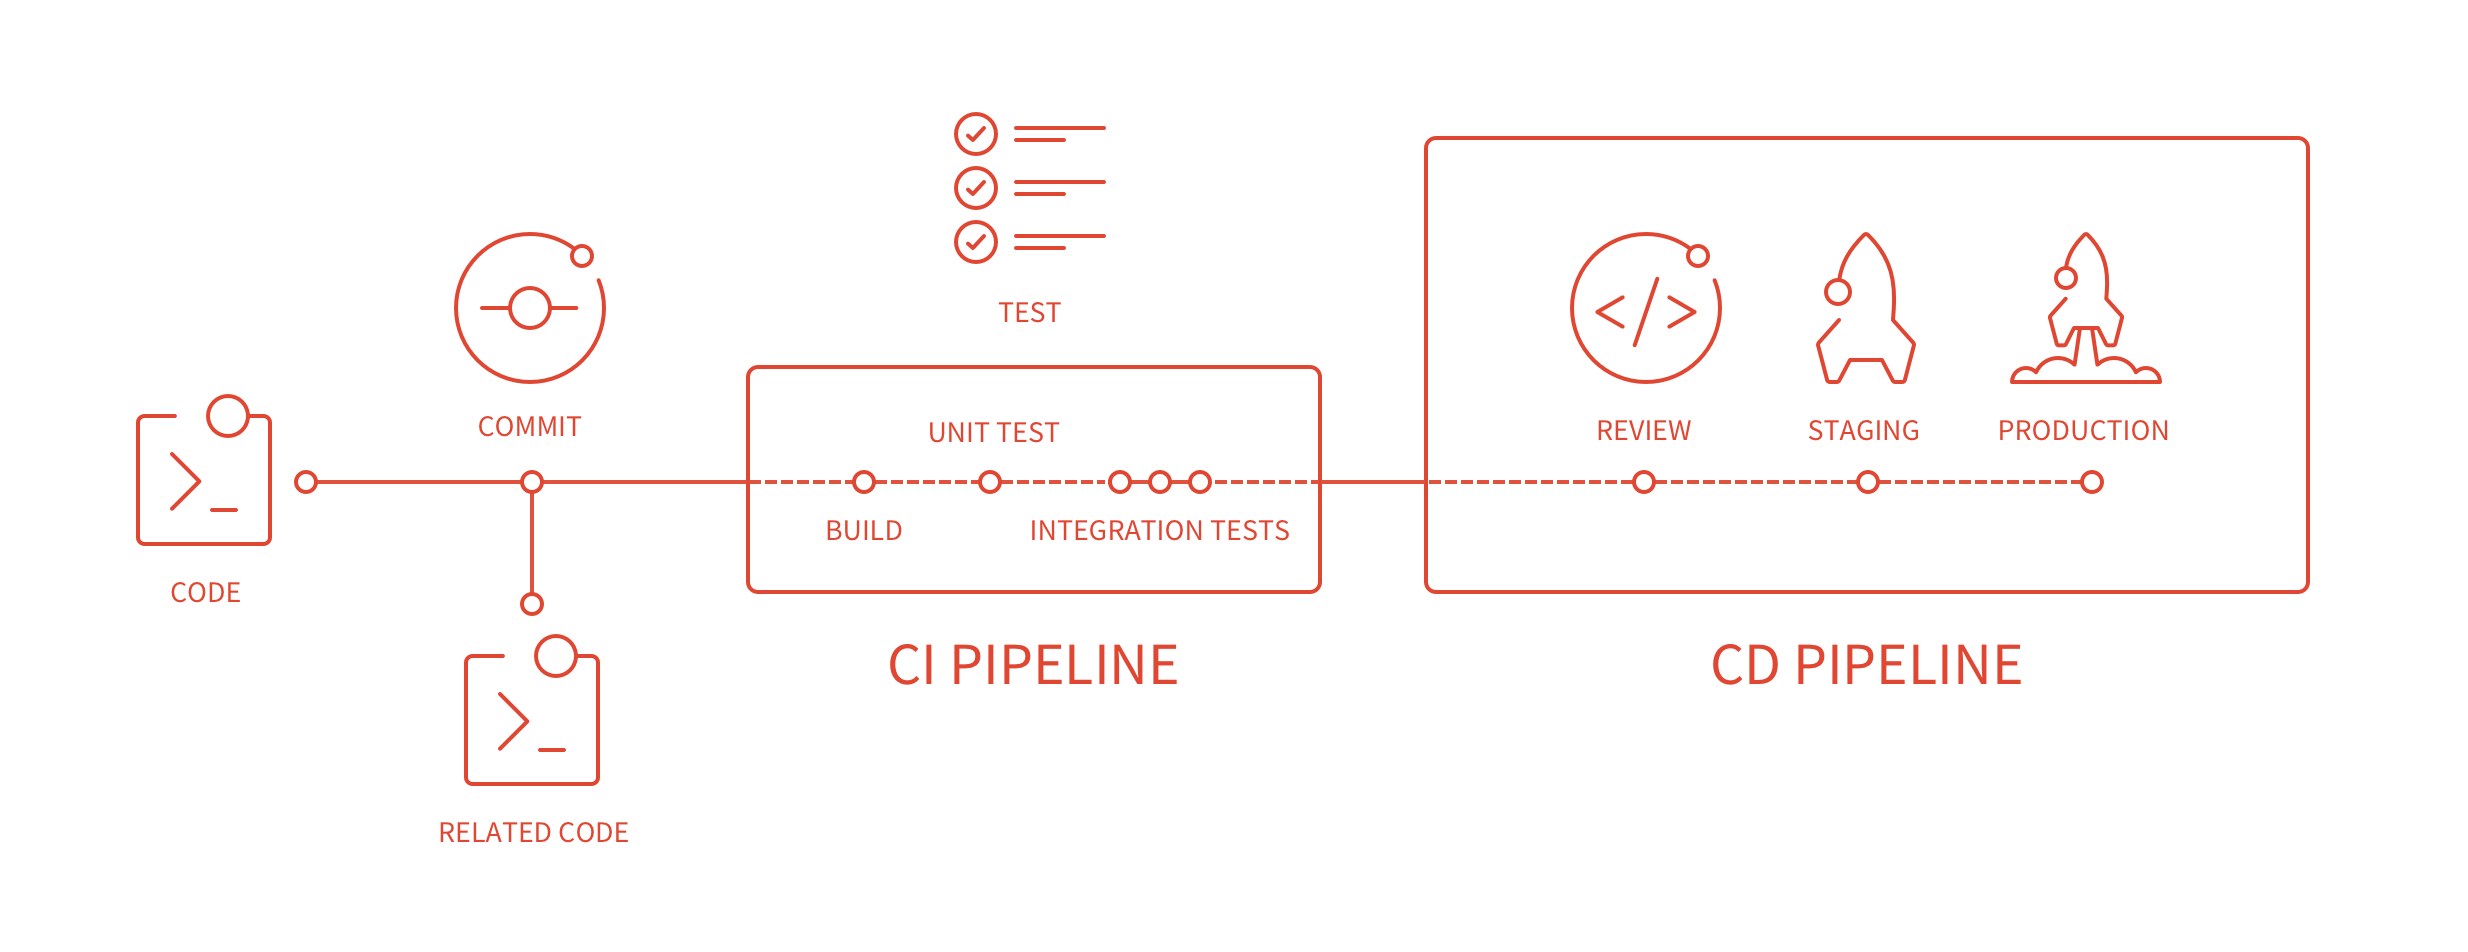
\includegraphics[scale=0.18]{./images/cicd_pipeline_gitlab.png}
		\caption{Rappresentazione del processo di CI/CD presso GitLab. Immagine dal sito web del produttore: \url{https://docs.gitlab.com/ee/ci/}}
	\end{center}
\end{figure}

\begin{figure}[H]
	\begin{center}
		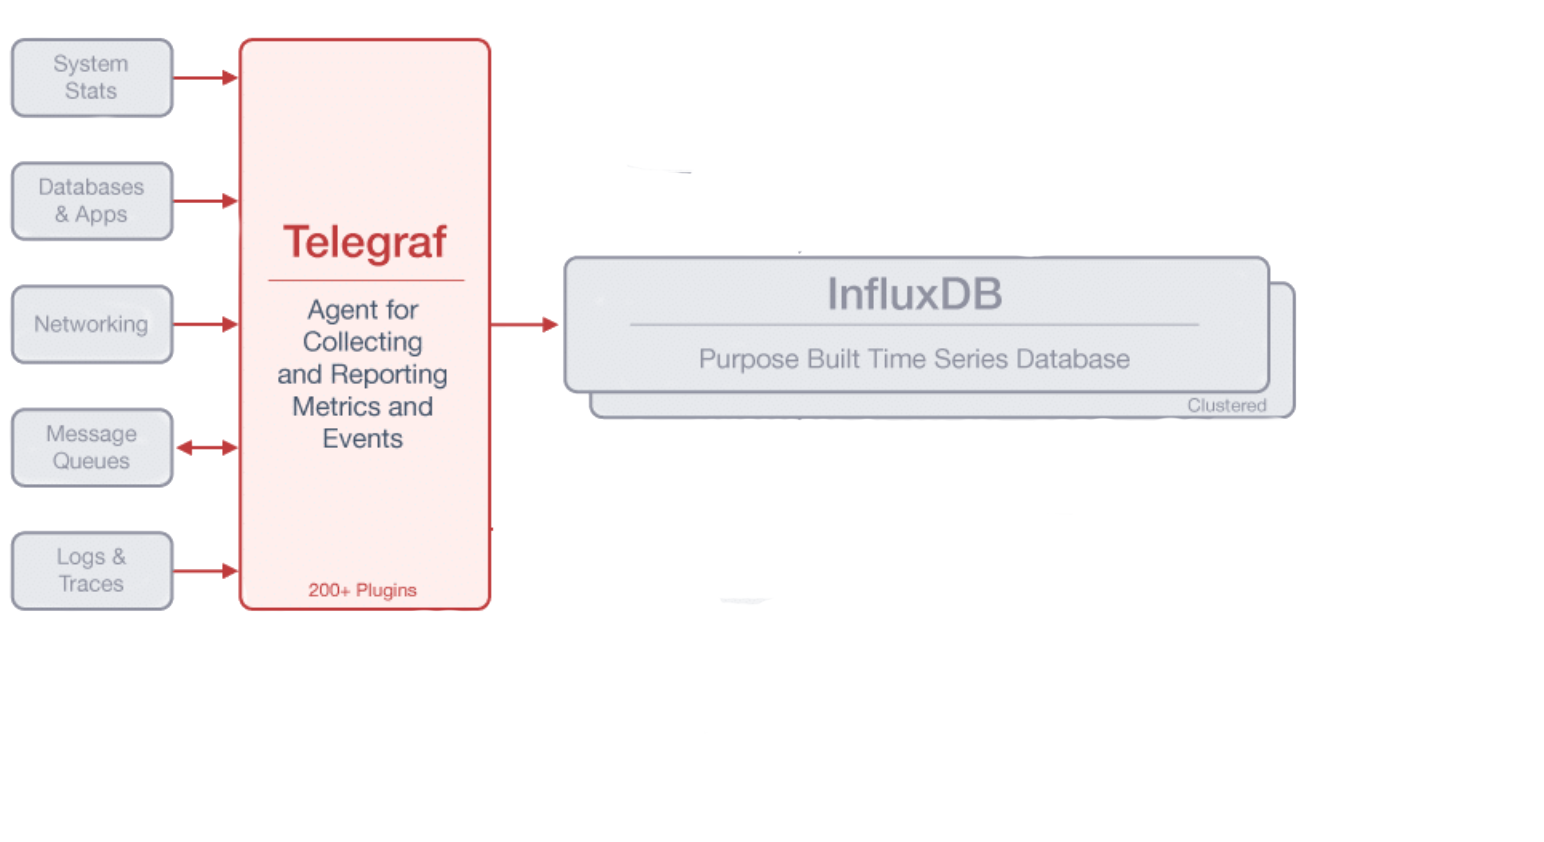
\includegraphics[scale=0.4]{./images/influxTelegraf.png}
		\caption{Rappresentazione del funzionamento di Telegraf e InfluxDB. Immagine dal sito web del produttore: \url{https://www.influxdata.com/time-series-platform/telegraf}}
	\end{center}
\end{figure}

\paragraph{Integrazione}\label{Progettazione_Integrazione}\-\\
L'attività di integrazione sarà effettuata utilizzando il servizio disponibile su \textit{GitLab}, piattaforma per repository utilizzata dal gruppo per il versionamento dei file sorgente.\\
Questo servizio implementa un modello di integrazione continua: ad ogni commit\glossario nel repository\glossario, \textit{GitLab} creerà automaticamente la build ed andrà ad eseguire i test di unità. In questo modo è possibile rilevare tempestivamente eventuali errori.\\
Per quanto riguarda il code coverage\glossario si utilizzerà un servizio messo a disposizione da \textit{GitLab}.\\

\paragraph{Diagrammi}\label{Progettazione_Diagrammi}\-\\
Per rendere più chiare le scelte progettuali adottate, si farà largo uso di diagrammi UML 2.0\glossario. Essi potranno essere di diversi tipi:
\begin{itemize}
	\item \textbf{Diagrammi dei Casi d'Uso}: dedicati alle funzionalità offerte dal sistema;
	\item \textbf{Diagrammi delle Classi}: dedicati alla descrizione degli oggetti che fanno parte del sistema, e le loro dipendenze;
	\item \textbf{Diagrammi dei Package}: dedicati alla descrizione delle dipendenze tra gli oggetti raggruppati in un package;
	\item \textbf{Diagrammi di Sequenza}: dedicati alla descrizione della collaborazione nel tempo tra un gruppo di oggetti;
	\item \textbf{Diagrammi di Attività}: dedicati ala descrizione della logica procedurale.
\end{itemize}

\paragraph{Obiettivi della Progettazione} \-\\
\label{Progettazione_Obiettivi}
La Progettazione serve per garantire che il prodotto sviluppato soddisfi le proprietà ed i requisiti delineati durante l'attività di analisi, ponendosi come obiettivi:
\begin{itemize}
	\item Garantire la qualità di prodotto sviluppato, perseguendo la correttezza per costruzione;
	\item Rendere chiara e comprensibile l'architettura progettata per gli stakeholder;
	\item Mantenere bassa la dipendenza tra le varie parti del prodotto favorendo la modularità ed il riuso;
	\item Ottimizzare l'uso delle risorse.
\end{itemize}

\subsubsection{Codifica}
Di seguito vengono definite delle norme che devono essere adottate dai \textit{Programmatori} per garantire una buona leggibilità  e manutenibilità  del codice. Le prime norme che seguiranno sono le più generali, da adottarsi per ogni linguaggio di programmazione adottato all'interno del progetto, in seguito quelle più specifiche per il linguaggio principale \textit{ECMAScript 6}\glossario.\\
Ogni norma è caratterizzata da un paragrafo di appartenenza, da un titolo, una breve descrizione e, se il caso lo richiede, un esempio.\\
Il rispetto delle seguenti norme è fondamentale per garantire uno stile di codifica uniforme all'interno del progetto, oltre che per massimizzare la leggibilità  e agevolare la manutenzione, la verifica\glossario e la validazione\glossario.

\paragraph{Convenzioni per i Nomi} \label{Nomi}
\begin{itemize}	
	\item I \textit{Programmatori} devono adottare come notazione per la definizione di cartelle, file, metodi, funzioni e variabili il CamelCase\glossario.\\
	Di seguito un esempio di corretta nomenclatura:
	\begin{lstlisting}[language=JavaScript]
//Cartelle 
./thisIsAFolder	//OK
./ThisIsAFolder //NO

//File
myFile.extension //OK
MyFile.extension //NO

//Funzioni
myFunction() { ... } //OK
MyFunction() { ... } //NO
	\end{lstlisting}

	\item Tutti i nomi devono essere unici ed autoesplicativi, ciò per evitare ambiguità  e limitare la complessità .
\end{itemize}
\paragraph{Convenzioni per la Documentazione}
\begin{itemize}	
	\item Tutti i nomi ed i commenti al codice vanno scritti in inglese;
	\item Nel codice è possibile utilizzare un commento con denominazione TODO in cui si vanno ad indicare compiti da svolgere;
	\item L'intestazione di ogni file deve essere la seguente:
	\begin{lstlisting}[language=JavaScript]
/**
* File: nameFile
* Type: fileType
* Creation date: yyyy-mm-gg
* Author: Name Surname
* Author e-mail: email@example.com
* Version: versionNumber 
*
* Changelog:
* #entry || Author || Date || Description
*/
	\end{lstlisting}
	\item La versione del file nell'intestazione deve rispettare la seguente formulazione: $X.Y.Z$, dove X rappresenta la versione principale, Y la versione parziale della relativa versione principale e Z l'avanzamento rispetto ad Y.\\ I numeri di versione del tipo $X.0.0$, dalla $1.0.0$, vengono considerate versioni stabili e quindi versioni da testare per saggiarne la qualità .
\end{itemize}
\paragraph{\textit{ECMAScript 6}}\label{EcmaScript6} \-\\
Seguendo le indicazioni presenti nella documentazione\footnote{\texttt{\url{http://docs.grafana.org/plugins/developing/development/}}} dell'azienda fornitrice di \textit{Grafana}, la piattaforma  per cui si intende sviluppare il plug-in, il team ha deciso di adottare come linguaggio di programmazione principale \textit{ECMAScript 6}\footnote{Linguaggio divenuto standard ISO: ISO/IEC 16262:2011, e relativo aggiornamento ISO/IEC 22275:2018.}.\\
\textit{ECMAScript 6} viene stardardizzato da \textit{ECMA}\glossario\ nel giugno 2015 con la sigla "ECMA-262".\\
Come stile di codifica si adottano le linee guida proposte da \textit{Airbnb JavaScript Style Guide}. Per la verifica dell'adesione a tali norme, i \textit{Programmatori} devono utilizzare, come suggerito dalla documentazione proposta da \textit{Grafana}, \textit{ESLint}\glossario.\\
In particolare i \textit{Programmatori} devono rispettare 5 linee guida proposte dalla documentazione ufficiale di \textit{Grafana}:
\begin{enumerate}
	\item Se una variabile non viene riutilizzata, deve essere dichiarata come \texttt{const};
	\item Utilizzare preferibilmente, per la definizione di variabili, la keyword  \texttt{let}, anziché  \texttt{var};
	\item Utilizzare il marcatore freccia (\texttt{\textbf{=>}}), in quanto non oscura il \texttt{this}:
	\begin{lstlisting}[language=JavaScript]
testDatasource() {
  return this.getServerStatus()
  .then(status => {
    return this.doSomething(status);
  })
}	
	\end{lstlisting}
	Invece che:
	\begin{lstlisting}[language=JavaScript]
testDatasource() {
  var self = this;
  return this.getServerStatus()
    .then(function(status) {
  return self.doSomething(status);
  })
}
	\end{lstlisting}
	\item Utilizzare l'oggetto \textit{Promise}:
	\begin{lstlisting}[language=JavaScript]
metricFindQuery(query) {
  if (!query) {
    return Promise.resolve([]);
  }
}	
	\end{lstlisting}
	Invece che:
	\begin{lstlisting}[language=JavaScript]
metricFindQuery(query) {
  if (!query) {
    return this.$q.when([]);
  }
}
	\end{lstlisting}
	%conseguenti?
	\item Se si utilizza \textit{Lodash}\glossario, per coerenza, lo si preferisca alle array function native di \textit{ES6}.
\end{enumerate}
Verranno esaminate di seguito le norme in merito allo stile di codifica che i \textit{Programmatori} dovranno adottare.

\subparagraph{Indentazione}\-\\
\textbf{Norma 1}\\
L'indentazione è da eseguirsi con tabulazione la cui larghezza sia impostata a due (2) spazi per ogni livello.\\
Di seguito un esempio da ritenersi corretto:
\begin{lstlisting}[language=JavaScript]
function() {
..let x = 2;
..if (x > 0)
....return true;
..else
....return false;
}
\end{lstlisting}
Qualsiasi altro tipo di indentazione è da ritenersi scorretta.\\
\-\\
\textbf{Norma 2}\\
Dopo la graffa principale va inserito uno (1) spazio. Nel seguente modo:
\begin{lstlisting}[language=JavaScript]
function() { ... }
\end{lstlisting}
\-\\
\textbf{Norma 3}\\
Dopo la keyword di un dato statement (\texttt{if, while}, etc.) va inserito uno (1) spazio. Per un esempio corretto si veda la norma successiva.\\
\-\\
\textbf{Norma 4}\\
Prima dell'apertura della graffa negli statement di controllo va inserito uno (1) spazio. Nel seguente modo:
\begin{lstlisting}[language=JavaScript]
function() {
  if (condition) {
    ...  
  }
  while (condition) {
    ...
  }
}
\end{lstlisting}
\-\\
\textbf{Norma 5}\\
Negli statement di controllo (\texttt{if, while}, etc.) le condizioni concatenate o annidate, mediante operatori logici, che diventano eccessivamente lunghe NON vanno espresse in un'unica linea, bensì spezzate in più righe. Nel seguente modo:
\begin{lstlisting}[language=JavaScript]
function() {
  if (condition && condition) {
    ...  
  }
  
  if (
   veryLongCondition
   && longCondition
   && condition
    ) {
    doSomething();
  }
}
\end{lstlisting}
\-\\
\textbf{Norma 6}\\
Dopo blocchi, o prima di un nuovo statement va lasciata una riga vuota. Nel seguente modo:
\begin{lstlisting}[language=JavaScript]
function1() {
  if (condition) {
    doSomething():  
  }
  
  return toReturn;  
}

function2(){
  ...
}
\end{lstlisting}
\-\\
\textbf{Norma 7}\\
I blocchi di codice multi-riga devono essere contenuti all'interno di graffe. Blocchi costituiti da una singola riga non è necessario che siano contenuti tra graffe: nel caso non vengano utilizzate, la definizione deve essere inline, cioè sulla stessa riga.\\
Nel seguente modo:
\begin{lstlisting}[language=JavaScript]
if (condition) return true;

if (condtion) {
  return true;
}
\end{lstlisting}

\subparagraph{Commenti al Codice}\-\\
\textbf{Norma 1}\\
Il codice va commentato nel seguente modo:
\begin{itemize}
	\item "\texttt{//}" se il commento occupa una sola riga;
	\item "\texttt{/** ... */} " se il commento occupa più righe.
\end{itemize}
Nel seguente modo:
\begin{lstlisting}[language=JavaScript]
// single line comment
if (condition) return true;

/**
* multi line comment, line 1
* multi line comment, line 2
*/
if (condtion) {
  return true;
}
\end{lstlisting}
\textbf{Norma 2}\label{Docs_Codice}\\
Il codice sviluppato va adeguatamente commentato con i commenti di documentazione appositi:
\begin{lstlisting}[language=JavaScript]
/**
 * Function or class description ...
 */
\end{lstlisting}
Il team fa riferimento a quanto indicato dal sito \textit{@use JSDoc}.\\
In particolari vengono ritenuti necessari, qualora utilizzato, il riferimento alle seguenti parti:
\begin{itemize}
	\item \textbf{@extends}: da utilizzare nell'intestazione della classe se la stessa ne estende un'altra;
	\item \textbf{@param}: da utilizzare per descrivere l'uso di un parametro di una funzione;
	\item \textbf{@return}: da utilizzare per descrivere il tipo di valore ritornato da una funzione; 
	\item \textbf{@module}: da utilizzare per indicare un modulo importato;
	\item \textbf{@throws}: da utilizzare per descrivere quali eccezioni possono essere lanciate.
\end{itemize}
Di seguito un esempio di utilizzo:
\begin{lstlisting}[language=JavaScript]
**
* Class representing a dot.
* @extends Point
*/
class Dot extends Point {
  /**
  * Create a dot.
  * @param {number} x - The x value.
  * @param {number} y - The y value.
  * @param {number} width - The width of the dot, in pixels.
  */
  constructor(x, y, width) {
    // ...
  }

  /**
  * Get the dot's width.
  * @return {number} The dot's width, in pixels.
  */
  getWidth() {
    // ...
  }
  
  /**
  * Set the dot's width.
  * @param {number} width - The width of the dot, in pixels.
  * @throws {Error} Will throw an error if the argument is lower than 0.
  */
  setWidth(w) {
    if(w < 0) throw new Error('Negative width');
    this.width = w;
  }
}
\end{lstlisting}

\subparagraph{Variabili}\-\\
\textbf{Norma 1}\\
Fare riferimento alle norme 1 e 2, all'inizio della sezione §\ref{EcmaScript6}.

\-\\
\textbf{Norma 2}\\
Non utilizzare dichiarazioni multiple di variabili, dichiarare una variabile per riga.\\
Nel seguente modo:
\begin{lstlisting}[language=JavaScript]
// OK
var x = 1;
var y = 0;

// NO
var x = 1, y = 0;
\end{lstlisting}


%va linkato il paragrafo
\subparagraph{Nomi}\-\\
\textbf{Norma 1}\\
 Oltre a quanto enunciato nel secondo punto del paragrafo §\ref{Nomi}, tutti i nomi di funzioni o variabili composti da una singola lettera, o che indichino temporaneità della variabile sono vietati: ogni nome deve essere significativo.\\
\-\\
\textbf{Norma 2} 
\begin{enumerate}
	\item I nomi delle variabili, funzioni ed istanze devono utilizzare il CamelCase;
	\item I nomi delle classi deve avere lo stile \texttt{capWords}.
\end{enumerate}
Nel seguente modo:
\begin{lstlisting}[language=JavaScript]
// OK
var thisIsAVariable;

function thisIsAFunction() { ... }

class ThisIsAClass() {
  ...
}

// NO
var Variable;

function Function() { ... }

class myClass() {
  ...
}
\end{lstlisting}

\paragraph{\textit{CSS}}
\label{css} \-\\
Per la parte front-end\glossario del plug-in il gruppo \texttt{Agents of S.W.E.} ha scelto di utilizzare i linguaggi \textit{CSS3}\glossario ed \textit{HTML5}\glossario.\\
Qui di seguito verrà descritta la Style Guide resa disponibile da \textit{Airbnb CSS-in-JavaScript Style Guide}.

\subparagraph{Indentazione} \-\\
\textbf{Norma 1}\\
Tra blocchi adiacenti dello stesso livello deve essere lasciata una linea bianca, tra l'una e l'altra. In questo modo il codice risulterà essere più leggibile. \\
Di seguito, un esempio della corretta indentazione: 


\begin{lstlisting} [language=JavaScript]
//OK
{
  bigBang: {
    display: 'inline-block',
    '::before': {
      content: "''",
    },
  },
  universe: {
    border: 'none',
  },
}

//NO
{
  bigBang: {
    display: 'inline-block',

    '::before': {
      content: "''",
    },
  },

  universe: {
    border: 'none',
  },
}
\end{lstlisting}

Per le restanti regole si farà riferimento allo standard imposto dalla World Wide Web Consortium\footnote{\href{http://www.w3.org/}{\texttt{W3C}}}. Per essere considerato corretto il file \textit{.css} dovrà essere validato tramite il sito reso disponibile dall'organizzazione, precedentemente nominata. La validazione potrà essere effettuata tramite il sistema messo a disposizione dalla W3C \footnote{\url{http://validator.w3.org/}}.

\paragraph{\textit{HTML}}
\label{html}\-\\

Insieme al \textit{CSS3}, per lo sviluppo della parte front-end del progetto, il gruppo ha scelto di utilizzare \textit{HTML5}. Per la stesura della Style Guide verrà utilizzata la documentazione resa disponibile da W3C.\\
Di seguito saranno riportate le principali norme da seguire: \\
	\textbf{Norma 1}\\
		Il tipo di documento deve sempre essere dichiarato all'inizio del documento, in maiuscolo o minuscolo a piacere; \\
	\textbf{Norma 2}\\
		I nomi degli elementi ed attributi devono essere sempre scritti in minuscolo; \\
	\textbf{Norma 3}\\
		Tutti gli elementi \textit{HTML} devono essere chiusi, anche se vuoti; \\
	\textbf{Norma 4}\\
		Il valore degli attributi deve essere racchiuso dentro doppio apice;\\
	\textbf{Norma 5}\\
		Intorno al simbolo di uguaglianza (=) non devono essere presenti spazi;\\
	\textbf{Norma 6}\\
		Devono essere usati due (2) spazi e non le tabulazioni. Gli spazi bianchi vanno utilizzati solamente per ampli blocchi di codice, per una maggiore leggibilità; \\
	\textbf{Norma 7}\\
		Nonostante i tag \texttt{html}, 	\texttt{body} e \texttt{head} possano essere omessi, vanno inseriti affinché siano compatibili con tutti i browser;\\
	\textbf{Norma 8}\\
		Le classi che verranno dichiarate all'interno dell'\textit{HTML}, al fine di andare poi a ridefinire il \textit{CSS}, dovranno essere quelle rese disponibili dalla documentazione di Grafana.	\\


Equivalentemente al \textit{CSS}, anche il codice \textit{HTML} dovrà essere validato. Questa validazione avverrà tramite il sito reso disponibile dalla W3C, al seguente \href{https://validator.w3.org/}{link}.

%AGGIUNGERE E SISTEMARE DA QUA IN GIU

\paragraph{\textit{AngularJS}} \label{angularjs} \-\\
Insieme al \textit{CSS} e all'\textit{HTML} il team ha deciso di sviluppare la parte front-end appoggiandosi al framework \textit{JavaScript Angularjs}\footnote{\url{https://www.angularjs.org/}}\glossario.\\
\textit{AngularJS} è un framework per applicazioni web, sviluppato con lo scopo di affrontare le difficoltà incontrate con lo sviluppo di applicazioni su singola pagina di tipo client-side. \-\\
La caratteristica principale è l'introduzione di funzionalità chiamate direttive, che permettono di creare componenti \textit{HTML} personalizzati e riusabili con lo scopo di associare a ogni direttiva un comportamento, così nascondendo la complessità della struttura DOM\glossario\. Le direttive sono riconoscibili poichè integrate nei tag con la dicitura "ng-" e susseguite dal nome (scelto dallo sviluppatore). 
Di seguito sono riportate alcune norme da seguire:\\
\textbf{Norma 1}\\
Verrà seguito il pattern Model View Controller(MVC)\glossario che propone la scomposizione in tre componenti:
\begin{itemize}
	\item \textbf{Model}: responsabile per il mantenimento e l'elaborazione dei dati;
	\item \textbf{View}: responsabile per la visualizzazione dei dati all'utente;
	\item \textbf{Controller}: si occupa di controllare l'interazione tra Model e View.
\end{itemize} 
\textbf{Norma 2}\\
Il controller non deve essere sovraccaricato di funzionalità che non gli appartengono. In particolare il controller non deve:
\begin{itemize}
	\item manipolare il DOM, questo renderà i controller difficili da testare. Questo compito è riservato alle direttive;
	\item formattare l'input, a questo scopo vengono usati i form \textit{Angular};
	\item formattare l'output, sarà compito dei filtri;
	\item condividere dati con altri controller;
	\item implementare funzionalità generali, le funzionalità che non riguardano direttamente l'interazione tra dati e la visualizzazione, deve essere fatta nei servizi.
\end{itemize}
\textbf{Norma 3}\\
Il nome dei moduli seguono la notazione lowerCamelCase;
\begin{lstlisting} [language=HTML]
	
	<div ng-app="myModule">...</div>

\end{lstlisting}
\textbf{Norma 4}\\
Quando è presente un modulo b che è submodule di a, si possono concatenere usando la notazione a.b;\\
\textbf{Norma 5}\\
Il nome dei controller viene assegnato in base alla loro funzionalità e viene usata la notazione UpperCamelCase;
\begin{lstlisting} [language=HTML]
	<div ng-controller="MyController">
  		{{ greeting }}
	</div>
\end{lstlisting}
\textbf{Norma 6}\\
I nomi delle restanti direttive seguono la notazione camelCase;
\begin{lstlisting} [language=HTML]
	<select class="myClass" ng-model="myModel">
\end{lstlisting}
\textbf{Norma 7}\\
Le direttive \textit{AngularJS} vengono scritte alla fine degli attributi di un tag: 
\begin{lstlisting} [language=HTML]
	//OK
	<p>Nome: <input type="text" ng-model="utente.nome"></p>
	
	//NO
	<p>Nome: <input ng-model="utente.nome" type="text"></p>
\end{lstlisting}
\textbf{Norma 8}\\
Il prefisso \$ è riservato ad \textit{AngularJS}, non deve essere usato per nomi di variabili, proprietà o metodi;\\
\textbf{Norma 9}\\
I controller non devono essere definiti globali;\\
\textbf{Norma 10}\\
Usare prefissi personalizzati per le direttive per evitare collisioni con librerie di terze parti;\\
\textbf{Norma 11}\\
In \textit{AngularJS} viene adottato il two-way binding, ogni modifica al modello dati si riflette sulla view e ogni modifica alla view viene riportata sul modello dati.
Questa sincronizzazione avviene senza la necessità di scrivere codice particolare, è sufficiente associare il modello allo scope all'interno del controller ed utilizzare la direttiva ng-model nella view.


\paragraph{\textit{WebStorm}}\-\\
Come software per lo sviluppo comune, il team ha scelto di utilizzare l'IDE \textit{WebStorm}, facente parte della famiglia di prodotti di JetBrains. \\
\textit{WebStorm} è una cross-platform, sviluppata principalmente per lo sviluppo web, \textit{JavaScript e TypeScript}. \\
La configurazione della piattaforma di sviluppo dovrà essere equivalente per tutti i componenti del gruppo. All'interno della piattaforma dovrà essere installato il plug-in \textit{ESLint}, la cui funzione verrà illustrata in seguito.

\paragraph{\textit{NPM}}\label{NPM} \-\\
\textit{Npm} è un gestore di pacchetti per \textit{JavaScript}, gestisce inoltre i pacchetti di default presenti nell'ambiente \textit{Node.js}\glossario.\\
Risulta essere strutturato in due parti: un client a riga di comando ed un database, contente pacchetti sia pubblici che privati. Lo scopo di \textit{node.js} è quello di incoraggiare il riuso del codice tra team ed il suo utilizzo è mirato alla gestione delle dipendenze.\\ 
Il suo utilizzo è necessario per poter eseguire e testare il codice \textit{ES6}.

\paragraph{\textit{ESLint}}\-\\
Il plug-in \textit{ESLint}, scaricabile dall'apposita sezione all'interno dell'IDE utilizzato, ha la funzione di segnalare errori che vengono effettuati durante la stesura del codice, in modo da evitare bug e rendere il codice più coerente. \\ 
Si occupa inoltre di far aderire il codice allo standard \textit{Airbnb} che il team ha deciso di adottare, segnalando le varie difformità.\\
Il plug-in è reperibile tra i pacchetti resi disponibili da \textit{NPM}\footnote{\url{https://www.npmjs.com/package/eslint}}.\\
Le regole utilizzate all'interno del plug-in saranno quelle esplicitate nella sezione §\ref{EcmaScript6}, riguardanti lo stile e le regole da rispettare per la stesura del codice con \textit{EcmaScript6}.

\paragraph{\textit{Jest}}\-\\
\label{jest}
\textit{Jest} è un framework per il testing di \textit{JavaScript} che il team ha deciso di adottare per la costruzione e l'esecuzione dei test di unità.\\
Inoltre, il framework offre la possibilità di eseguire il calcolo del code coverage dei file testati.

\paragraph{\textit{Webpack}} \label{webpack}\-\\
\textit{Webpack} è un module bundler\glossario per applicazioni \textit{javascript}. Nella pratica lo scopo di \textit{webpack} è creare un pacchetto di assets leggibile e utilizzabile dal browser a partire da un insieme di file sorgenti strutturati su diversi file e con dipendenze complesse. \\
Gli aspetti fondamentali sono:
\begin{itemize}
\item \textbf{Entry Point}: rappresenta il punto di partenza da cui iniziare la build e creare lo schema delle dipendenze, di default è './src/index.js' ma può essere modificato nei file di configurazione;
\item \textbf{Output}: rappresenta la destinazione in cui verranno generati i file leggibili dal browser, di default è './dist' e il file principale è './dist/main.js';
\item \textbf{Loaders}: di default \textit{webpack} esegue la build solamente di file \textit{javascript} e \textit{JSON}\glossario, tramite questa configurazione \textit{webpack} può essere adattato ad altri tipi di file, così da permettere la conversione anche di essi. I loaders possono avere due proprietà: 
	\begin{itemize}
	\item La proprietà test che identifica quali file dovrebbero essere trasformati;
	\item La proprietà use che identifica quali loaders utilizzare per eseguire la trasformazione.
	\end{itemize}
\item \textbf{Plugins}: a differenza dei loaders, i plugins operano in aspetti più generali riguardanti l'ottimizzazione dei pacchetti e la gestione delle risorse. Per utilizzare un plugin bisogna eseguire una 'require' dalla sorgente ed aggiungerlo mediante la 'new' nell'array apposito chiamato 'plugin'.
\item \textbf{Mode}: viene settato in base all'ambiente in cui lanciato \textit{webpack}, cosi da importare ottimizzazioni specifiche. Può assumere i seguenti valori:
	\begin{itemize}
	\item Development;
	\item Production;
	\item None.
	\end{itemize}
Se non viene specificato viene settato come valore di default 'production'.
\end{itemize}

 






\subsection{Ambiente di Test del Prodotto}\label{Server}
Il team \texttt{Agents Of S.W.E.} ha deciso, per avere un ambiente comune su cui testare il prodotto in via di sviluppo, di dotarsi di un server noleggiato online attraverso la nota piattaforma di hosting \textit{DigitalOcean}.\\
Il server in oggetto è raggiungibile all'indirizzo IP \texttt{142.93.102.115} ha le seguenti caratteristiche:
\begin{itemize}
	\item SO: Ubuntu 18.04 LTS;
	\item CPU: 1x Intel(R) Xeon(R) CPU E5-2650 v4 @ 2.20GHz;
	\item RAM: 2GiB ECC DIMM;
	\item SSD: 24GiB.
\end{itemize}
Il team ha provveduto ad installare all'interno del server i seguenti pacchetti:
\begin{itemize}
	\item \textit{Grafana};
	\item \textit{InfluxDB};
	\item \textit{Telegraf};
	\item \textit{Apache}\glossario.
\end{itemize}
